\documentclass{standalone}
\usepackage{tikz}
\usepackage{ctex,siunitx}
\usepackage{tkz-euclide}
\usepackage{amsmath}
\usetikzlibrary{patterns, calc}
\usetikzlibrary {decorations.pathmorphing, decorations.pathreplacing, decorations.shapes,}
\begin{document}
\small
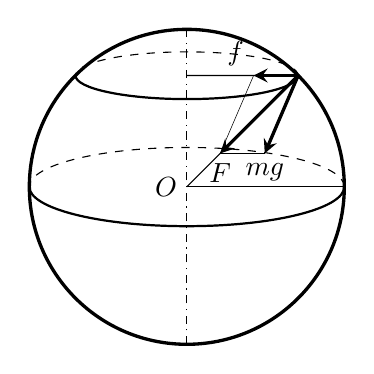
\begin{tikzpicture}[>=stealth,scale=1]
  \tkzDefPoints{0/0/O, 1.414/1.414/S}
  \draw[very thick](O) circle (2);
  \draw[dashed] (O) ellipse[x radius=2, y radius=.5];
  \draw[dashed] (0,1.414) ellipse[x radius=1.414, y radius=.3];
  \draw[dashdotted](0,-2)--(0,2);
  \draw(O)--(2,0);
  \draw(0,1.414)--(S)--(O);
  \tkzDefPoints{0/1.414/S_1}
  \tkzDefPointWith[linear, K=.4](S,S_1) \tkzGetPoint{f}
  \tkzDefPointWith[linear, K=.7](S,O) \tkzGetPoint{F}
  \tkzDefPointsBy[translation = from f to S](F){F'}
  \tkzDrawSegments[very thick, ->](S,f S,F S,F')
  \tkzDrawSegments(F,f F,F')
  \tkzLabelPoints[left](O)
  \tkzLabelPoints[above left](f)
  \tkzLabelPoint[below](F'){$mg$}
  \tkzLabelPoints[below](F)
  \draw[thick](2,0) arc [start angle =0, end angle =-180, x radius=2, y radius=.5];
  \draw[thick](S) arc [start angle =0, end angle =-180, x radius=1.414, y radius=.3];
\end{tikzpicture}
\end{document}